As previously established, the robot must remain inside $\mathcal{B}$ to enforce safety. Based on that, at each subproblem solve, we use the state solution of Problem \ref{problem:mi} to compute the predicted healthiness (PH) index $\lambda \vcentcolon (0,\|\alpha\|) \mapsto (0, 1)$, our blending mechanism. More precisely, we measure how far the robot is from violating the boundary of the working conditions within a virtual horizon whose length is defined as $N_b \leq N$. Then, we select an index $\lambda$ between 0 and 1 that is used to determine the actual weighting in Problem \ref{problem:mi}. Note that the weighting matrices have a clear and direct relationship with the MI controller behavior: the closer the index is to 0, the more the weighting to follow the motion generator commands; conversely, the closer the index is to 1, the more the weighting to follow the human inputs. 

Moreover, the fact that $N_b$ may differ from $N$ introduces much flexibility in the controller's design. It allows one to determine the level of insight that the blending mechanism should have into the interaction, as we will see in simulation. In what follows, we formally define the PH index.
\begin{definition}[PH index] \normalfont Given a virtual horizon with $N_b$ intervals and the predicted $\eta_i$ from the state solution of Problem \ref{problem:mi}, let us first select the largest excursion within $\mathcal{B}$ 
	\begin{equation}
		d_{\rm max} = \max_{i=0,\dots,N_b}\|\eta_i-\eta^r_i\|.
	\end{equation}
Then, to ensure that the PH index is a strictly positive function in the range of interest, let us consider a saturation function $d_{\rm sat} \vcentcolon [0, \|\alpha\|] \mapsto (0, \|\alpha\|)$ defined by the following Richards growth curve
\begin{align}
		&d_{\rm sat}(d_{\rm max}, \Lambda) \vcentcolon = \nonumber\\
		&\frac{\mu_1\|\alpha\|}{(1 + \zeta \cdot \exp\{-\theta_2(d_{\rm max}-\mu_2\|\alpha\|)\})^{1/\zeta}} \in (0, \|\alpha\|),\label{eq:d_sat}
\end{align}
where $\Lambda = (\mu_1, \mu_2, \theta_2, \zeta)$ is a quadruple that parameterizes the Richards' curve (see Fig.~\ref{fig:d_sat}). In particular, $\mu_1$ is a constant related to the the upper asymptote and whose value is close to $1$ but strictly less than $1$, $\mu_2$ is a positive real number related to the lag phase, $\theta_2$ is the growth rate, and $\zeta$ is a positive real number known as the shape parameter\footnote{The shape of the curve $d_{\rm sat}$ is due to parameter $\zeta$. If $\zeta = 1$, one has the \emph{logistic function}. If $\zeta$ tends to zero, the curve converges to the \emph{Gompertz function}.}.

Finally, the PH index is defined as
\begin{equation}
		\lambda(d_{\rm sat}) \vcentcolon = \frac{\sqrt{\|\alpha\|^2 - d_{\rm sat}^2}}{\|\alpha\|}\in (0,1).\label{eq:ph_index}
\end{equation}
\end{definition} 

\noindent An illustration of function \eqref{eq:ph_index} is provided in Fig.~\ref{fig:ph_index}. Its profile indicates the aggressiveness with which the MI controller decreases human control authority. In particular, when $d_{\rm sat}$ is extremely high, the controller should be more belligerent and heavily ignore human inputs. 

\begin{figure}[t]
\centering
	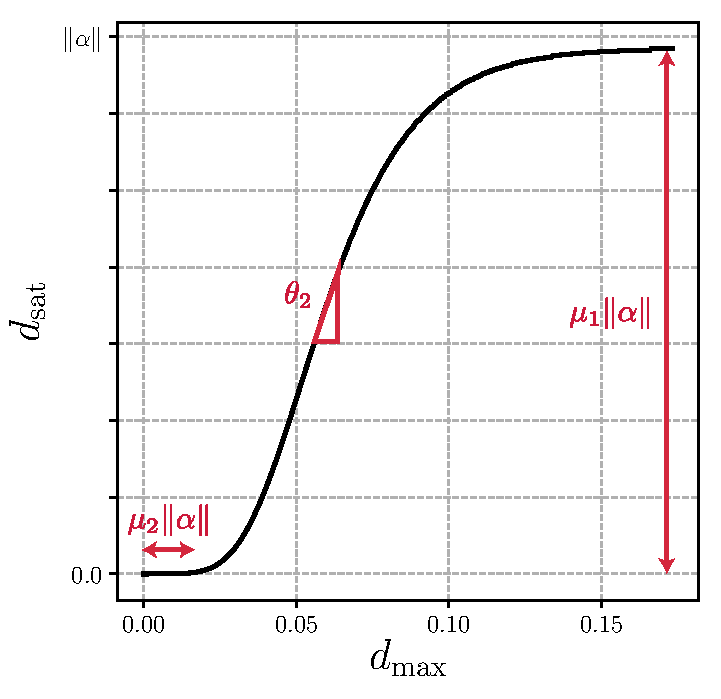
\includegraphics[width=.35\textwidth]{figures/dsat_edited}
	\vspace{-0.35cm}
	\caption{Pictorial description of the saturation function \eqref{eq:d_sat}. Note that when $d_{\rm max} = \|\alpha\|$ then $d_{\rm sat} = \mu_1\|\alpha\|$.}\label{fig:d_sat}%
\end{figure}

\begin{figure}[t]
\centering
	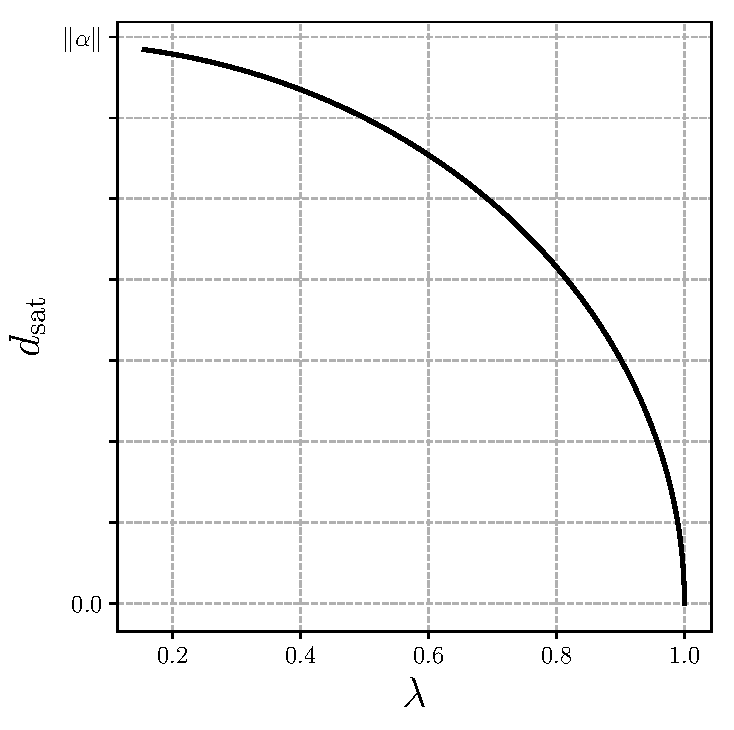
\includegraphics[width=.35\textwidth]{figures/decay_fcn}
	\vspace{-0.35cm}
	\caption{An illustration of the function defined in \eqref{eq:ph_index} showing a profile relatively quadratic for penalizing excursions inside $\mathcal{B}$.}\label{fig:ph_index}%
\end{figure}